\documentclass[11pt]{article}
\usepackage[margin=1in]{geometry}
\usepackage{amsmath}
\usepackage{booktabs}
\usepackage{graphicx}
\usepackage{caption}
\usepackage{subcaption}
\usepackage[hidelinks]{hyperref}
\usepackage{setspace}
\usepackage[T1]{fontenc}
\usepackage[utf8]{inputenc}
\usepackage{threeparttable}
\onehalfspacing
\graphicspath{{../output/figures/}}
\newcommand{\FSpooledFive}{0.992}
\newcommand{\FSpooledTen}{0.992}
\newcommand{\AcceptRF}{0.3}
\newcommand{\AcceptSE}{0.4}
\newcommand{\AcceptP}{0.55}
\newcommand{\AcceptMean}{98.3}
\newcommand{\RetainTwoRF}{0.6}
\newcommand{\RetainTwoP}{0.20}
\newcommand{\RetainFourRF}{0.7}
\newcommand{\RetainFourP}{0.35}
\newcommand{\DirectorRF}{1.0}
\newcommand{\DirectorP}{0.31}
\newcommand{\DirectorMean}{14.0}
\newcommand{\SameschRF}{-0.5}
\newcommand{\SameschSE}{0.7}
\newcommand{\SameschMean}{97.0}
\newcommand{\PromotedRF}{-2.7}
\newcommand{\PromotedP}{0.26}
\newcommand{\AcceptFifteenRF}{1.4}
\newcommand{\AcceptFifteenP}{0.20}
\newcommand{\RetainTwoFifteenRF}{1.5}
\newcommand{\RetainTwoFifteenP}{0.06}
\newcommand{\NombSixFifteenRF}{1.2}
\newcommand{\NombSixFifteenP}{0.36}
\newcommand{\DensityPooledP}{0.43}
\newcommand{\RuralSameschRF}{-2.6}
\newcommand{\RuralSameschSE}{1.3}
\newcommand{\RuralSameschP}{0.05}
\newcommand{\RuralSameschTwoRF}{-2.1}
\newcommand{\RuralSameschTwoP}{0.09}
\newcommand{\UrbanSameschRF}{0.5}
\newcommand{\RuralRetainRF}{-0.1}
\newcommand{\RuralRetainP}{0.83}
\newcommand{\PrimAcceptRF}{1.2}
\newcommand{\PrimAcceptP}{0.06}
\newcommand{\PrimRetainRF}{1.6}
\newcommand{\PrimRetainP}{0.03}
\newcommand{\FemRetainRF}{0.8}
\newcommand{\FemRetainP}{0.09}
\newcommand{\RuralUrbanDiff}{-3.1}
\newcommand{\RuralUrbanDiffSE}{1.5}
\newcommand{\RuralUrbanDiffT}{-2.1}
\newcommand{\InruralRuralRF}{-2.2}
\newcommand{\InruralRuralP}{0.08}
\newcommand{\InruralRuralMean}{96.3}
\newcommand{\UrbanRetainRF}{1.2}
\newcommand{\UrbanRetainP}{0.04}
\newcommand{\RuralRetainTwoRF}{-0.1}
\newcommand{\RuralOneSameschRF}{-5.1}
\newcommand{\RuralOneSameschP}{0.03}


% Marked pointers to where additional data would strengthen the analysis
\newcommand{\dataneed}[1]{\par\medskip\noindent\begin{small}\noindent
$\triangleright$~\textbf{More data would help here:} \emph{#1}\end{small}\par\medskip}

\title{The Bono de Atracci\'on and Teacher Retention in Peru:\\
Regression Discontinuity Evidence\\[6pt]
\large Working notes -- first results, data inventory, and next steps}
\author{Gianmarco Le\'on-Ciliotta\thanks{These notes were prepared with research
assistance from Claude (Anthropic). All data work is documented in the
accompanying code (\texttt{code/01}--\texttt{04}); nothing in the source data
folders was modified. Comments and corrections are very welcome.}}
\date{July 16, 2026}

\begin{document}
\maketitle

\begin{abstract}
\noindent We study the effects of Peru's \emph{Bono de Atracci\'on}---an
unconditional-on-location bonus of S/\,18,000 (about USD~4,800) paid over
three years to teachers who enter the permanent public-school career
(nombramiento) in the top third of their cohort's final merit ranking---on
position take-up, retention, and early-career progression. We exploit the
sharp discontinuity in bonus eligibility at the top-third cutoff of the final
concurso score, pooling the 2015, 2017, 2018 and 2019 national hiring
concursos (33,383 winners, of whom 11,147 received the bonus). Assignment is
essentially deterministic: crossing the cutoff raises the probability of
receiving the bonus from 0 to \FSpooledTen. Take-up of the permanent position
is nearly universal on both sides of the cutoff (\AcceptMean\% just below),
leaving little room for effects on the extensive margin: the RD estimate on
being on the public payroll the year after the concurso is
+\AcceptRF~percentage points (pp) and statistically indistinguishable from
zero. Retention point estimates are uniformly positive but small and
imprecise (+\RetainTwoRF~pp at $t+2$, $p=$~\RetainTwoP; +\RetainFourRF~pp at
$t+4$), with the clearest signal in the 2015 cohort---the only one we can
follow for six years (+\RetainTwoFifteenRF~pp at $t+2$,
$p=$~\RetainTwoFifteenP). We find a precise zero on remaining in the school
where the teacher was appointed, consistent with the rule that the bonus
follows the teacher rather than the school. The aggregate zero masks
offsetting responses: among winners assigned to \emph{rural} schools,
recipients are less likely to remain in their assigned school
(\RuralSameschRF~pp at $t+1$, $p=$~\RuralSameschP) and in the rural system
altogether (\InruralRuralRF~pp at $t+2$), while the aggregate retention gain
is concentrated among urban appointees (+\UrbanRetainRF~pp,
$p=$~\UrbanRetainP)---the windfall appears to finance the move out of
hard-to-staff schools. These notes document the institutional rules, the data inventory,
the identification checks, and a plan to extend the analysis to the 2022 and
2024 concursos and to richer outcomes; marked pointers throughout indicate
where additional data would most strengthen the analysis.
\end{abstract}

\section{Motivation and summary}

Attracting high-ability candidates into the teaching profession---and keeping
them there---is a first-order concern for education systems in developing
countries. A growing literature studies pay reforms and location-based
incentives for teachers, but surprisingly little is known about
\emph{selective} financial incentives that reward entering the profession at
the top of the ability distribution, holding the job and its location fixed.
Peru's \emph{Bono de Atracci\'on} is exactly such a policy: teachers who enter
the Carrera P\'ublica Magisterial (CPM) in the top third of the final merit
ranking of their national hiring concurso receive S/\,6,000 per year during
their first three years of service, conditional on remaining active permanent
teachers---anywhere in the public system.

These notes report a first pass at the question using a regression
discontinuity (RD) design around the top-third cutoff. Our reading of the
evidence so far is threefold. First, the design works mechanically very well:
the running variable (the unbonified final concurso score) assigns the bonus
essentially deterministically once the tie-broken mass point at the cutoff
score is set aside, and standard validity checks (density, covariate balance)
raise no red flags. Second, the margin the bonus was named for---attracting
winners into actually taking the position---has virtually no room to move:
about \AcceptMean\% of winners just below the cutoff appear on the public
payroll as permanent teachers the following year. Third, the interesting
action is in \emph{where} teachers stay rather than \emph{whether} they
stay: same-school retention---the margin the bonus does \emph{not} pay
for---shows a precise zero on aggregate, but the zero masks offsetting
responses. Rural appointees who receive the bonus become less likely to
remain in their assigned school ($p=$~\RuralSameschP) and in any rural
school, without leaving the profession, while the aggregate retention gain
(+\UrbanRetainRF~pp at $t+2$, $p=$~\UrbanRetainP) is entirely an
urban-appointee phenomenon: the bonus appears to finance exit from exactly
the schools where retention is scarce.
Sections~\ref{sec:institutions}--\ref{sec:results} document
these results; Sections~\ref{sec:dataplan}--\ref{sec:ideas} lay out the data
we still need and how the project could become a paper.

\section{Institutional background}\label{sec:institutions}

\subsection{Entry into the permanent teaching career}

Since the 2012 Ley de Reforma Magisterial (Ley 29944), entry into a permanent
public-school teaching position (\emph{nombramiento}) occurs exclusively
through national concursos. Each concurso has two stages. In the national
stage, all applicants take the Prueba \'Unica Nacional (PUN), a centralized
exam; those clearing minimum scores become \emph{habilitados} for the
decentralized stage, in which they apply to specific schools and are evaluated
locally (professional background, a classroom observation, and an interview).
The final score is the sum of the two stages, and winners
(\emph{ganadores})---applicants ranked first for a specific vacancy---receive
a nombramiento resolution and take up their plaza the following school year.
Concursos with a bono round were held in 2015, 2017, 2018, 2019, 2022 and
2024; this draft uses the first four, for which we have complete rankings
microdata (Table~\ref{tab:rounds}).

\subsection{The Bono de Atracci\'on}

Article 22 of Ley 30281 (the 2015 budget law) created a bonus for teachers
``who enter the Carrera P\'ublica Magisterial occupying the top third of the
final merit ranking of the public nombramiento concursos.'' The rules are laid
out in RM 666-2018-MINEDU and, since April 2021, in RVM 118-2021-MINEDU.
The features that matter for our design and interpretation are the following.

\begin{enumerate}
\item \textbf{Amount and timing.} S/\,6,000 per year for three consecutive
years, starting the year after the concurso, paid each December through the
regional payroll units. The total, S/\,18,000, is roughly seven months of the
entry-level teacher salary. The bonus is neither pensionable nor
remunerative.
\item \textbf{Eligibility.} The top third is computed \emph{nationally},
across all levels and specialties, among concurso winners registered as
\emph{nombrado} in the NEXUS payroll system at a validation date, excluding
teachers who were awarded the bonus in a previous concurso. The count of
eligible winners is divided by three (rounded) and the bonus goes to the top
of the ranking. Under the 2015--2019 rounds the ranking used the total
(final) concurso score; under RVM 118-2021---which governs the 2022 and 2024
rounds---the ranking uses the PUN score only. In both regimes the ranking
score \emph{excludes} the percentage bonifications (disability, armed forces)
that are added for plaza-allocation purposes.
\item \textbf{Conditionality.} Each annual payment requires (i) an active
nombramiento, (ii) at least five months of effective classroom service during
the school year (verified by the UGEL each September~15), and (iii) not having
been removed from the CPM. Crucially, service may be \emph{in any public
school}---transfers (reasignaciones) do not void the bonus. Missed years are
not recovered; resignation, dismissal or nullity of the appointment forfeits
all remaining payments.
\end{enumerate}

Point 3 shapes what we should expect: the bonus pays teachers to remain
permanent public-school teachers during their first three years, but it does
\emph{not} pay them to remain in the (often rural, hard-to-staff) school where
they were appointed. Effects on same-school retention would therefore have to
operate through an income effect or through selection, not through the
explicit incentive.

\dataneed{Two institutional details remain unverified and are worth an
information request to MINEDU (DIBRED): the exact tie-breaking rule applied at
the cutoff score, and the NEXUS validation dates used to define the eligible
pool in each round. Both matter for the handful of observations at and just
above the cutoff (Section~\ref{sec:data}).}

\begin{table}[htbp]
\centering
\caption{Concurso rounds, winners, and the top-third cutoff}
\label{tab:rounds}
\begin{threeparttable}
\begin{tabular}{lccccc}
\toprule
Concurso & Winners & Bono recipients & Share & Cutoff score & Payroll horizon \\
\midrule
2015 & 8,137  & 2,702 & 33.2\% & 228.0 & $t+1,\dots,t+6$ \\
2017 & 10,759 & 3,611 & 33.6\% & 227.5 & $t+1,\dots,t+4$ \\
2018 & 9,975  & 3,348 & 33.6\% & 224.0 & $t+1,\dots,t+3$ \\
2019 & 4,512  & 1,486 & 32.9\% & 222.0 & $t+1,t+2$ \\
2022 & --     & 9,999\tnote{a} & -- & -- & (data plan, Section~\ref{sec:dataplan}) \\
2024 & --     & 8,210\tnote{a} & -- & -- & (data plan, Section~\ref{sec:dataplan}) \\
\bottomrule
\end{tabular}
\begin{tablenotes}\footnotesize
\item Winners: ganadores with an adjudicated plaza in the cleaned concurso
files. Bono recipients: rows in the digitized beneficiary lists matched to
winners by DNI ($\geq$99.8\% match). Cutoff: minimum unbonified final score
among recipients. Payroll horizon: years relative to the concurso observable
in the NEXUS 2015--2021 annual extraction.
\item[a] Beneficiary list counts; concurso rankings not yet digitized.
\end{tablenotes}
\end{threeparttable}
\end{table}

\section{Data}\label{sec:data}

\subsection{Sources}

We combine three administrative sources, all matched by national ID (DNI).

\textbf{Bono beneficiary lists.} MINEDU publishes the list of beneficiaries
for each round; we digitized the PDFs into CSVs (2,702; 3,617; 3,351; 1,489;
9,999; and 8,210 names for 2015--2024). The 2015 list reports the final score
and the national merit rank; the 2017 list reports both the concurso score
(with bonifications) and the score used for the bono ranking; the 2018--2019
lists report the total score; the 2022 and 2024 lists report a score on a
different scale, consistent with the PUN-only ranking rule in
RVM~118-2021. Appendix~\ref{app:lists} records our file-by-file reading of
these lists and the open questions.

\textbf{Concurso rankings.} For 2015--2019 we have cleaned microdata covering
all 288,757 registered applicants (PUN scores), the 86,807 habilitados, the
153,779 decentralized-stage records (including sub-scores, bonifications, and
the assigned school), and the 33,383 winners. Winners merge to the bono lists
by DNI at $\geq$99.8\%.

\textbf{NEXUS payroll.} The Sistema de Administraci\'on y Control de Plazas
records every teaching position in the country. We use an annual (Nov/Dec)
national extraction for 2015--2021 (3.07 million position-year records) with
the incumbent's DNI, appointment status (nombrado/contratado/designado),
school code, position type, and pay scale (escala magisterial). This is the
same system MINEDU itself uses to validate bono payments.

\subsection{The running variable and the cutoff}

For 2015--2019 the bono ranking score is the final concurso score
\emph{excluding} law-mandated percentage bonifications. In the winners file
the recorded final score embeds those bonifications for about 2\% of winners;
we verified that for all 217 bono recipients whose recorded score differs from
the score on the beneficiary list, the gap equals exactly the sum of the
bonification sub-scores recorded in the decentralized-stage file. We therefore
use the unbonified score throughout. With this correction, assignment is
essentially deterministic: \emph{no} recipient lies strictly below the
round-specific cutoff (the minimum recipient score), and only 87 of 22,236
non-recipient winners (0.4\%) lie strictly above it---consistent with the
norm's exclusions (winners without a validated nombramiento at the cut-off
date, and prior beneficiaries).

One feature requires care: the cutoff score itself is a mass point where
eligibility was resolved by a tie-breaking rule we do not observe (at the 2015
cutoff score, 56 of 81 winners received the bonus; at the 2018 cutoff score,
only 4 of 99 did). Our baseline specification therefore drops the cutoff-score
mass point (a ``donut'' of one score value); estimates including it, treating
eligibility as fuzzy, are reported as robustness and are very similar.

\subsection{Outcomes}

For each winner we construct, from the payroll: (i) \emph{acceptance},
an indicator for appearing as nombrado in the November/December payroll the
year after the concurso; (ii) \emph{retention}, the same indicator at
$t+2,\dots,t+6$; (iii) \emph{same-school retention}, being nombrado in the
school where the concurso assigned them; (iv) \emph{career progression},
having advanced beyond the entry pay scale by 2021 and ever holding a
director/directivo position. Winners absent from the payroll in a given year
are coded zero for that year.

\dataneed{The binding data constraint for the whole project is the payroll
horizon: the NEXUS extraction ends in 2021, which truncates the 2018--2019
cohorts at $t+3$/$t+2$ and rules out the 2022/2024 cohorts entirely
(Section~\ref{sec:dataplan}, item 4). Two NEXUS panel files in the Dropbox
remain online-only placeholders
(\texttt{nexus\_panel\_teacher\_long\_new.dta},
\texttt{nexus\_panel\_teacher\_wide\_new.dta}); they are not needed for the
current results but should be synced before we rebuild anything that uses
them. Finally, monthly (rather than Nov/Dec) NEXUS snapshots---which exist in
the raw sources for some years---would let us measure within-year exits and
the exact five-month service condition MINEDU verifies.}

\section{Empirical strategy}\label{sec:design}

We compare concurso winners just above and just below their round's top-third
cutoff. Let $r_{ic}$ denote winner $i$'s unbonified final score centered at
the cutoff of concurso $c$. We estimate, pooling rounds and using
\texttt{rdrobust} (local linear, triangular kernel, MSE-optimal bandwidths,
robust bias-corrected inference),
\begin{equation}
y_{ic} = \alpha + \tau\,\mathbf{1}\{r_{ic} \geq 0\} + f(r_{ic}) + \varepsilon_{ic},
\end{equation}
where $f(\cdot)$ is estimated separately on each side of the cutoff. Because
assignment is deterministic in the donut sample, the reduced form and the
fuzzy RD (instrumenting bonus receipt with cutoff crossing) coincide up to the
0.4\% of protocol exclusions; we report both.

Two features make the design unusually credible. First, the cutoff is
determined \emph{ex post} by the realized distribution of scores---the number
of winners divided by three---so applicants could not target an unknown
threshold even if they could manipulate scores. Second, everyone in the sample
already won a permanent position, so both sides of the cutoff face identical
job offers; the only discontinuity is the S/\,18,000. Consistent with this,
the density of the running variable is smooth through the cutoff (pooled
$p=$~\DensityPooledP) and predetermined covariates (sex, age, rurality of the
assigned school, baseline payroll status) are balanced
(Table~\ref{tab:validity}, Figure~\ref{fig:balance}).

\section{Results}\label{sec:results}

\subsection{First stage}

Figure~\ref{fig:fs} shows the share of winners on the beneficiary list by
half-point score bins, by round and pooled. The probability of receiving the
bonus jumps from 0 to \FSpooledTen{} at the cutoff (local linear,
$\pm$10-point bandwidth, donut sample; Table~\ref{tab:firststage}). The
first stage is, for all practical purposes, one.

\begin{figure}[htbp]
\centering
\begin{subfigure}[b]{0.42\textwidth}
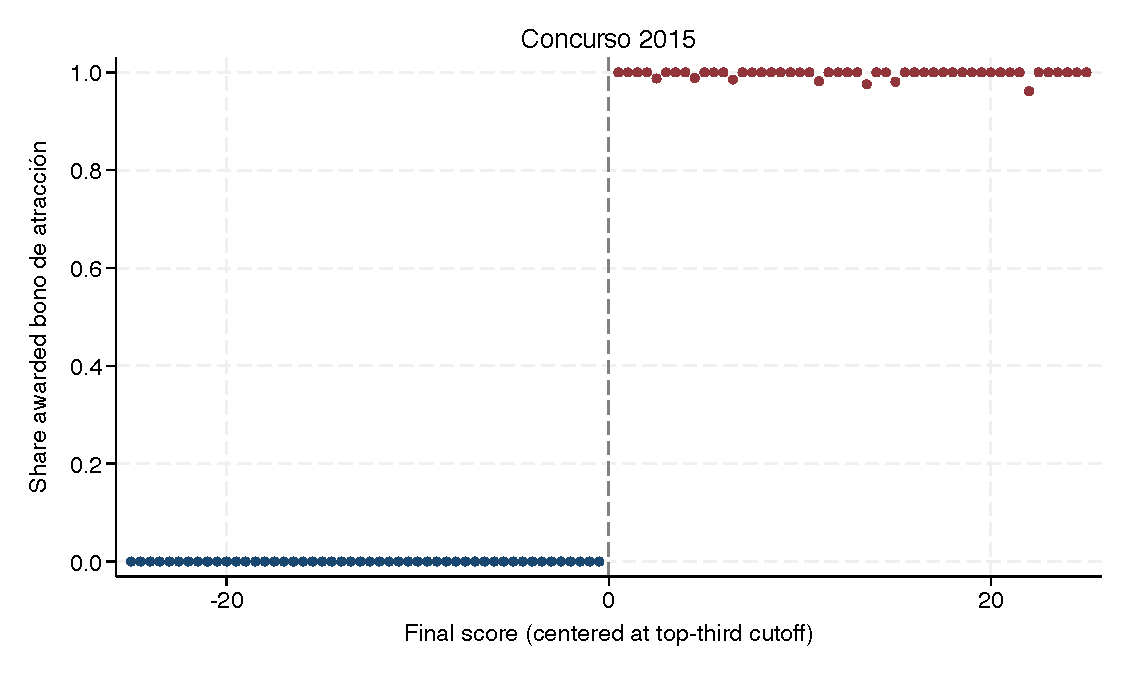
\includegraphics[width=\textwidth]{fig_fs_2015.pdf}
\end{subfigure}
\begin{subfigure}[b]{0.42\textwidth}
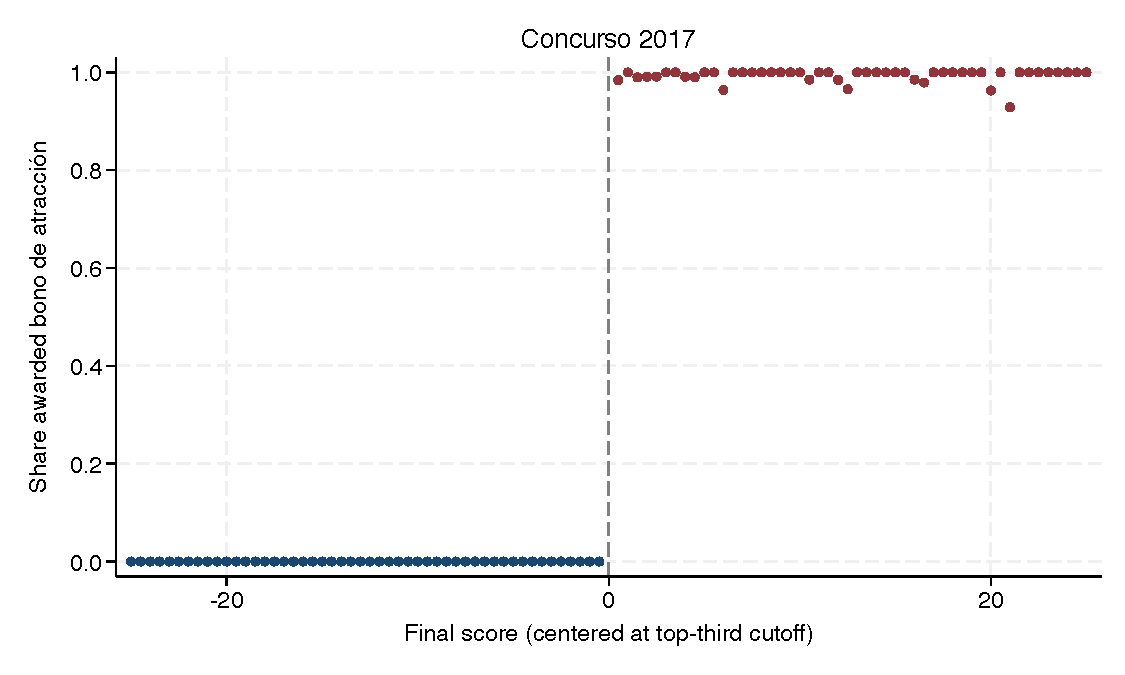
\includegraphics[width=\textwidth]{fig_fs_2017.pdf}
\end{subfigure}\\
\begin{subfigure}[b]{0.42\textwidth}
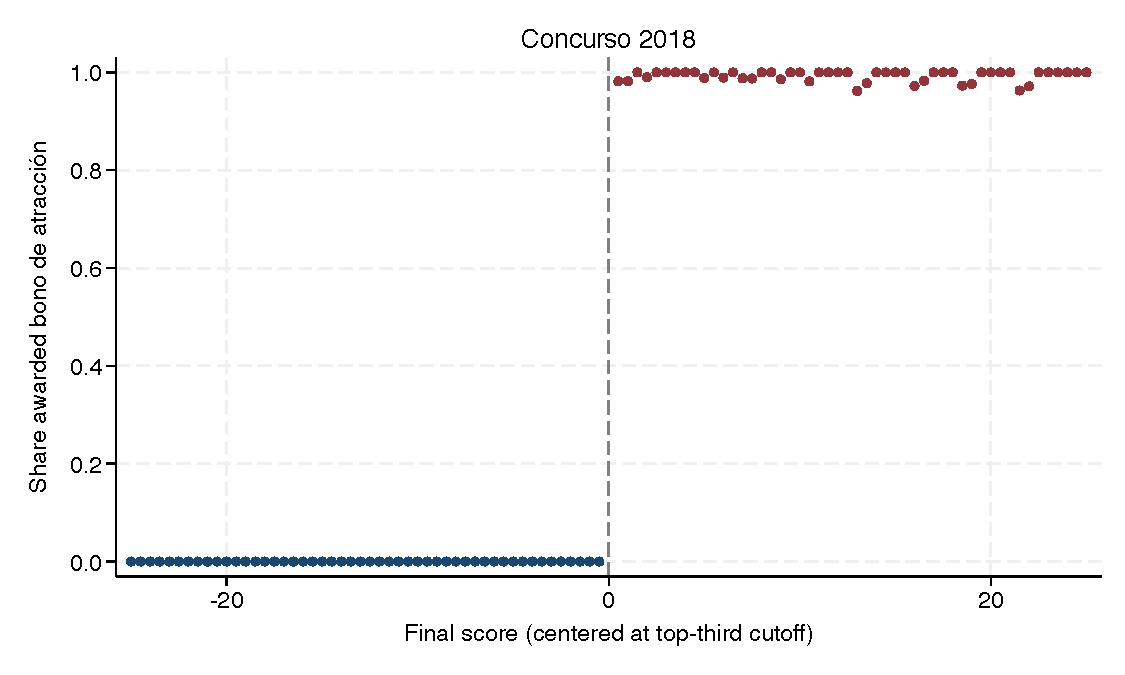
\includegraphics[width=\textwidth]{fig_fs_2018.pdf}
\end{subfigure}
\begin{subfigure}[b]{0.42\textwidth}
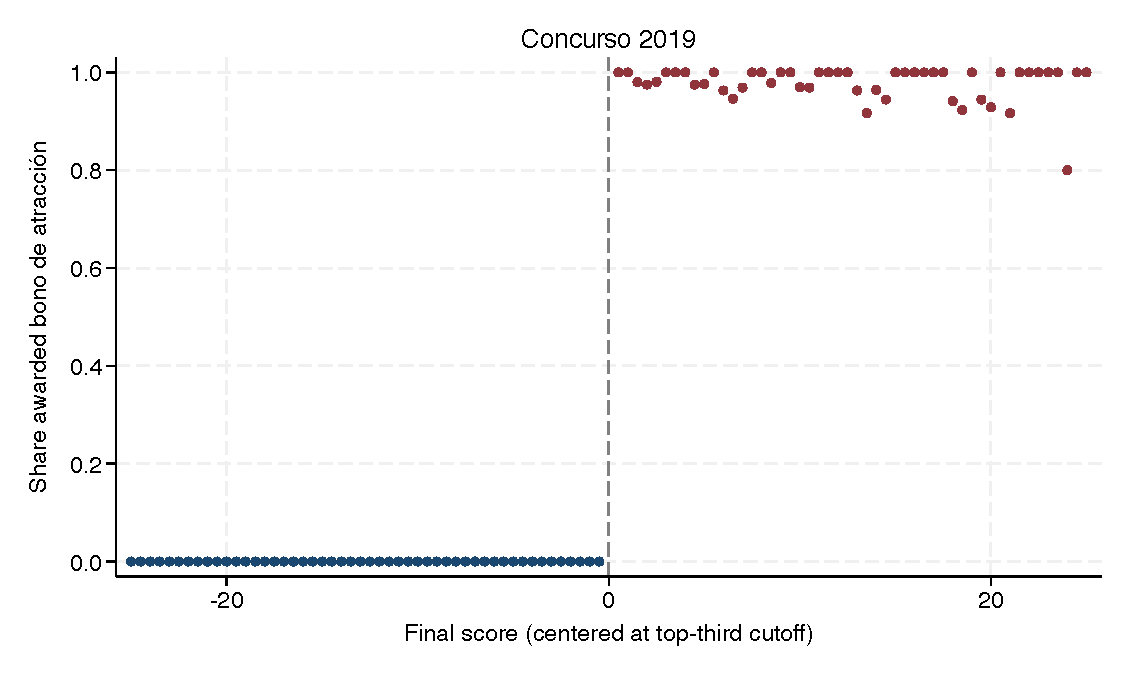
\includegraphics[width=\textwidth]{fig_fs_2019.pdf}
\end{subfigure}\\
\begin{subfigure}[b]{0.5\textwidth}
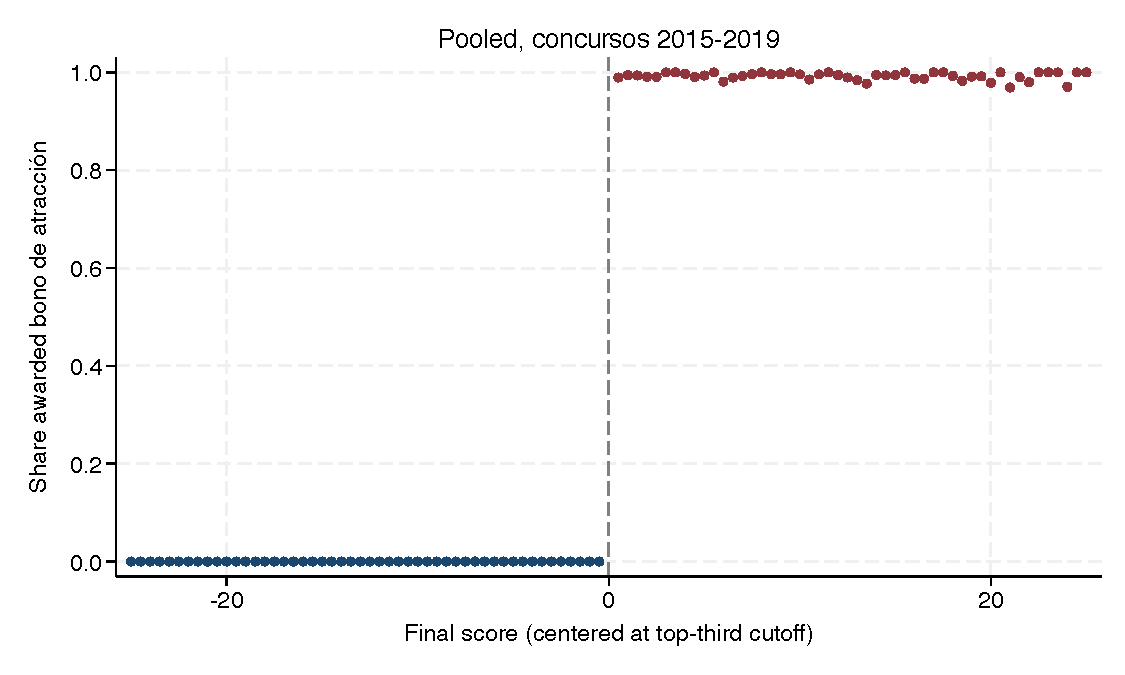
\includegraphics[width=\textwidth]{fig_fs_pooled.pdf}
\end{subfigure}
\caption{First stage: probability of receiving the Bono de Atracci\'on.
Half-point bins of the unbonified final score, centered at the round-specific
top-third cutoff; the tie-broken cutoff-score mass point is excluded.}
\label{fig:fs}
\end{figure}

\begin{table}[htbp]
\centering
\caption{First-stage estimates (donut sample)}
\label{tab:firststage}
\begin{threeparttable}
\begin{tabular}{lccccc}
\toprule
 & 2015 & 2017 & 2018 & 2019 & Pooled \\
\midrule
\multicolumn{6}{l}{\emph{Bandwidth $\pm5$ points}} \\
RD estimate & 1.000 & 0.990 & 0.986 & 0.994 & 0.992 \\
 & (0.002) & (0.006) & (0.008) & (0.010) & (0.003) \\
Obs.\ left/right & 984/823 & 1261/1107 & 1095/942 & 542/444 & 3882/3316 \\
\midrule
\multicolumn{6}{l}{\emph{Bandwidth $\pm10$ points}} \\
RD estimate & 0.997 & 0.990 & 0.991 & 0.991 & 0.992 \\
 & (0.002) & (0.004) & (0.004) & (0.007) & (0.002) \\
Obs.\ left/right & 2016/1503 & 2575/2013 & 2281/1746 & 1092/792 & 7964/6054 \\
\bottomrule
\end{tabular}

\begin{tablenotes}\footnotesize
\item Local linear regression of bonus receipt on an above-cutoff indicator,
the centered score, and their interaction, within the indicated bandwidth,
excluding the cutoff-score mass point. Robust standard errors in parentheses.
\end{tablenotes}
\end{threeparttable}
\end{table}

\subsection{Acceptance and retention}

Take-up of the position is close to universal on both sides of the cutoff:
\AcceptMean\% of winners in the five points below the cutoff are nombrados on
the public payroll the following November. The RD estimate is
+\AcceptRF~pp (robust $p=$~\AcceptP; Table~\ref{tab:outcomes},
Figure~\ref{fig:outcomes}). Permanent positions in Peru are valuable enough
that essentially every winner takes one; there is simply no margin for the
bonus to move here. The same holds for being on the payroll under any
status.

Retention estimates are uniformly positive but small and individually
insignificant: +\RetainTwoRF~pp at $t+2$ ($p=$~\RetainTwoP) and
+\RetainFourRF~pp at $t+4$ ($p=$~\RetainFourP), against a control mean around
98\%. The dynamics are displayed in Figure~\ref{fig:dynamics}. The clearest
signal comes from the 2015 cohort, the only one we can follow six years out:
+\RetainTwoFifteenRF~pp at $t+2$ ($p=$~\RetainTwoFifteenP) and
+\NombSixFifteenRF~pp at $t+6$ ($p=$~\NombSixFifteenP). With attrition from
the CPM this low, even a bonus of seven months' salary can at most move
retention by a point or two---the ceiling is the story. Still, two readings
of the positive pattern remain open, and we cannot yet separate them: a
genuine retention effect concentrated among the few would-be leavers, or
noise. The horizon extension to 2022--2025 payroll data
(Section~\ref{sec:dataplan}) will help, both by adding the 2018--2019
cohorts' post-payment years (if the effect is incentive-driven, it should
plateau or fade once payments stop) and by adding statistical power.

Same-school retention shows no discontinuity at any horizon
(\SameschRF~pp at $t+1$, SE \SameschSE, on a base of \SameschMean\%):
recipients are no more likely to stay in the school that appointed them. This is exactly what
the rules predict---the bonus follows the teacher, not the school---and it
suggests the policy purchases system-level retention (already near its
ceiling) rather than retention where scarcity actually binds. We consider
this one of the most policy-relevant facts so far, and
Section~\ref{sec:hetero} pushes on it by splitting the sample by the rurality
of the assigned school.

\dataneed{Extending the payroll to 2022--2025 does double duty in this
section: it adds the post-payment years for the 2018--2019 cohorts (the test
for whether the retention effect fades when the money stops) and it roughly
doubles the pooled sample at horizons $t+3$ and beyond, where the point
estimates are largest but the confidence intervals are widest.}

\subsection{Career progression}

Neither career outcome moves robustly. Marginal recipients are
+\DirectorRF~pp more likely to ever hold a director/directivo position by
2021 ($p=$~\DirectorP), on a control mean of \DirectorMean\%; the estimate
was larger and marginally significant before excluding the tie mass point
(+2.6~pp, $p=0.06$, fuzzy), so we flag it as worth revisiting with the
directivo concurso files (which we have) rather than payroll job codes alone.
Progression beyond the entry pay scale by 2021 shows a noisy negative
estimate (\PromotedRF~pp, $p=$~\PromotedP, 2015/2017 cohorts), which we do
not over-interpret; ascenso opportunities were limited and cohort-specific.

\dataneed{Career outcomes are currently inferred from payroll job codes and
pay scales alone. The ascenso concurso results (2018, 2019, 2021) and the
directivo concurso files (habilitados and ganadores, already in
\texttt{concursos/clean}) would let us measure \emph{attempted} versus
\emph{achieved} promotion separately---the margin an income windfall should
move first. Administrative salary data (SUP/planillas) would also let us put
a soles value on each career transition and calibrate the income effect.}

\begin{table}[htbp]
\centering
\caption{RD estimates: acceptance, retention, and career outcomes (pooled)}
\label{tab:outcomes}
\begin{threeparttable}
\small
\begin{tabular}{lcccccc}
\toprule
 & \multicolumn{2}{c}{Reduced form} & \multicolumn{2}{c}{Fuzzy RD} & & Control \\
\cmidrule(lr){2-3}\cmidrule(lr){4-5}
Outcome & Estimate & (SE) & Estimate & (SE) & $N$ (bw) & mean \\
\midrule
Nombrado in payroll, $t+1$ (acceptance) & 0.003 & (0.004) & 0.003 & (0.004) & 18,694 & 0.983 \\
Nombrado, $t+2$ & 0.006 & (0.004) & 0.006 & (0.004) & 16,388 & 0.983 \\
Nombrado, $t+3$ & 0.006 & (0.004) & 0.006 & (0.004) & 15,223 & 0.983 \\
Nombrado, $t+4$ & 0.007 & (0.007) & 0.007 & (0.007) & 7,758 & 0.981 \\
In payroll (any status), $t+1$ & -0.000 & (0.004) & -0.000 & (0.004) & 13,398 & 0.990 \\
In payroll (any status), $t+2$ & 0.002 & (0.004) & 0.002 & (0.004) & 12,739 & 0.991 \\
In payroll (any status), $t+3$ & 0.002 & (0.004) & 0.002 & (0.004) & 12,134 & 0.990 \\
Nombrado in assigned school, $t+1$ & -0.005 & (0.007) & -0.005 & (0.007) & 13,398 & 0.970 \\
Nombrado in assigned school, $t+2$ & -0.001 & (0.007) & -0.001 & (0.007) & 17,010 & 0.961 \\
Nombrado in assigned school, $t+3$ & -0.003 & (0.009) & -0.003 & (0.009) & 13,190 & 0.950 \\
Ever director/directivo by 2021 & 0.010 & (0.011) & 0.010 & (0.011) & 18,694 & 0.140 \\
Escala 2+ by 2021 (2015/17 cohorts) & -0.027 & (0.024) & -0.027 & (0.024) & 8,450 & 0.395 \\
\bottomrule
\end{tabular}

\begin{tablenotes}\footnotesize
\item Donut sample (cutoff-score mass point excluded). \texttt{rdrobust}
local linear estimates, triangular kernel, MSE-optimal bandwidth; robust
bias-corrected $p$-values: * $p<0.1$, ** $p<0.05$, *** $p<0.01$. Control mean:
outcome mean for winners 0--5 points below the cutoff. Fuzzy RD instruments
bonus receipt with cutoff crossing. Horizons $t+3$ ($t+4$) exclude the 2019
(2018--19) cohorts.
\end{tablenotes}
\end{threeparttable}
\end{table}

\begin{table}[htbp]
\centering
\caption{RD estimates by cohort (donut sample, reduced form)}
\label{tab:cohorts}
\begin{threeparttable}
\begin{tabular}{lcccc}
\toprule
 & 2015 & 2017 & 2018 & 2019 \\
\midrule
Nombrado, $t+1$ & 0.014 & 0.001 & -0.008 & 0.016 \\
 & (0.011) & (0.008) & (0.009) & (0.010) \\
Nombrado, $t+2$ & 0.015* & 0.002 & 0.000 & 0.014 \\
 & (0.008) & (0.008) & (0.008) & (0.010) \\
\midrule
Nombrado, $t+4$ & 0.012 & 0.002 & -- & -- \\
 & (0.009) & (0.008) & -- & -- \\
Nombrado, $t+5$ & 0.007 & -- & -- & -- \\
 & (0.011) & -- & -- & -- \\
Nombrado, $t+6$ & 0.012 & -- & -- & -- \\
 & (0.012) & -- & -- & -- \\
\bottomrule
\end{tabular}

\begin{tablenotes}\footnotesize
\item \texttt{rdrobust} local linear estimates by concurso; standard errors
in parentheses; * $p<0.1$, ** $p<0.05$, *** $p<0.01$ (robust bias-corrected).
Later horizons only observable for earlier cohorts given payroll through
2021.
\end{tablenotes}
\end{threeparttable}
\end{table}

\begin{figure}[htbp]
\centering
\begin{subfigure}[b]{0.42\textwidth}
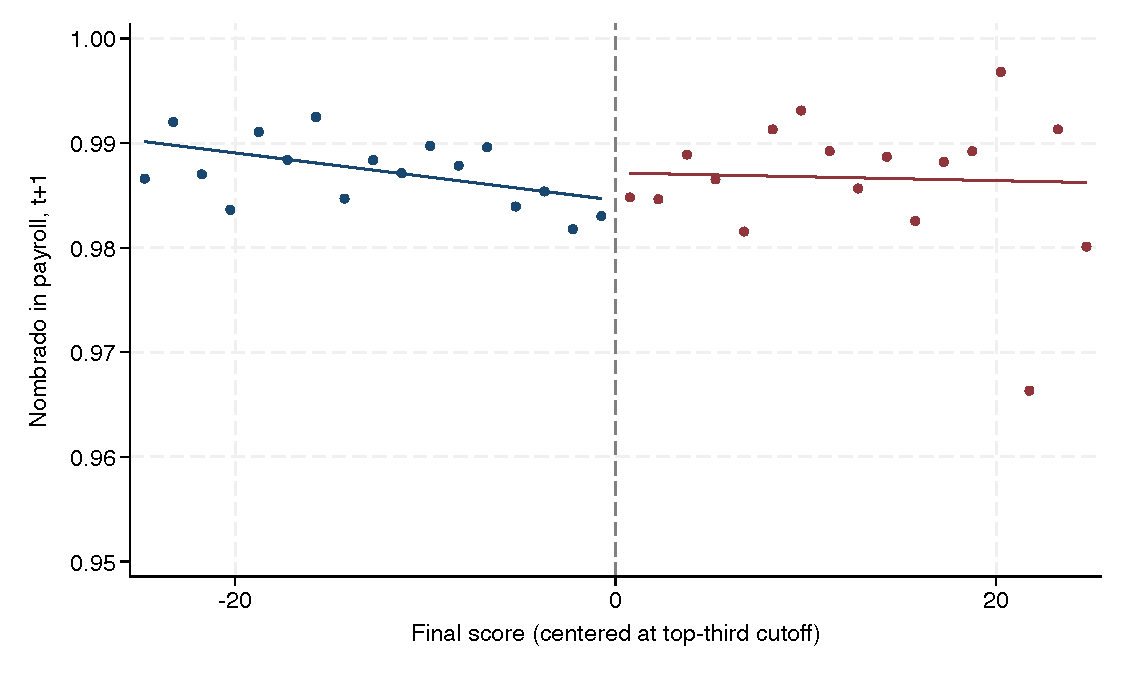
\includegraphics[width=\textwidth]{fig_rf_accept.pdf}
\caption{Nombrado, $t+1$}
\end{subfigure}
\begin{subfigure}[b]{0.42\textwidth}
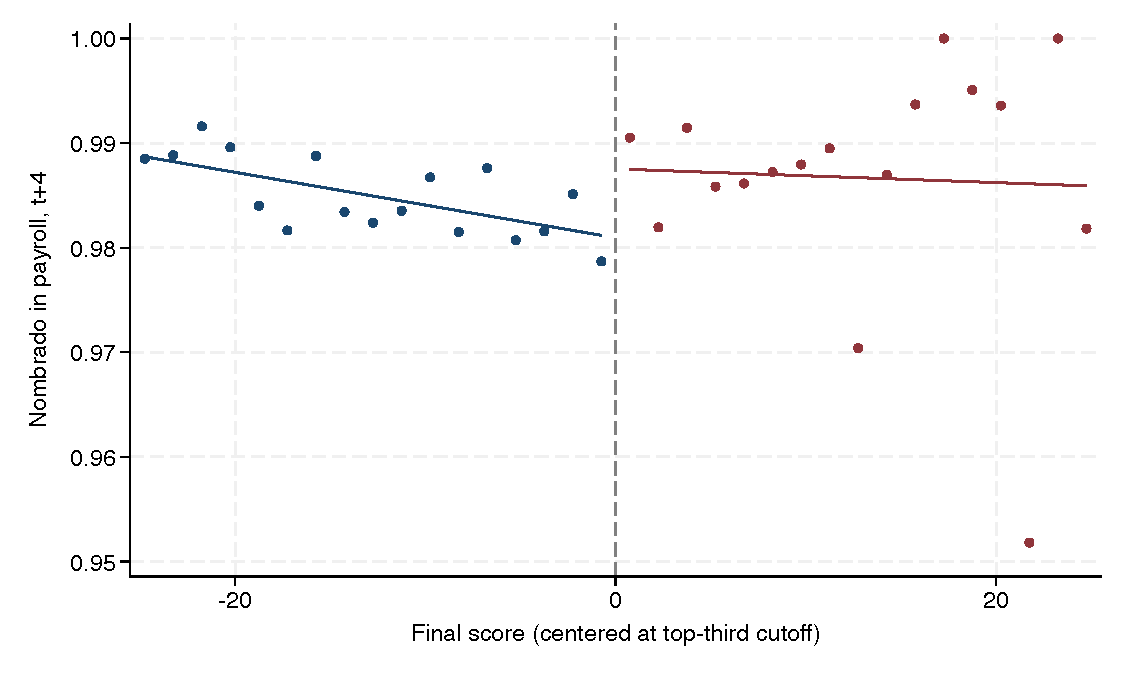
\includegraphics[width=\textwidth]{fig_rf_retain4.pdf}
\caption{Nombrado, $t+4$}
\end{subfigure}\\
\begin{subfigure}[b]{0.42\textwidth}
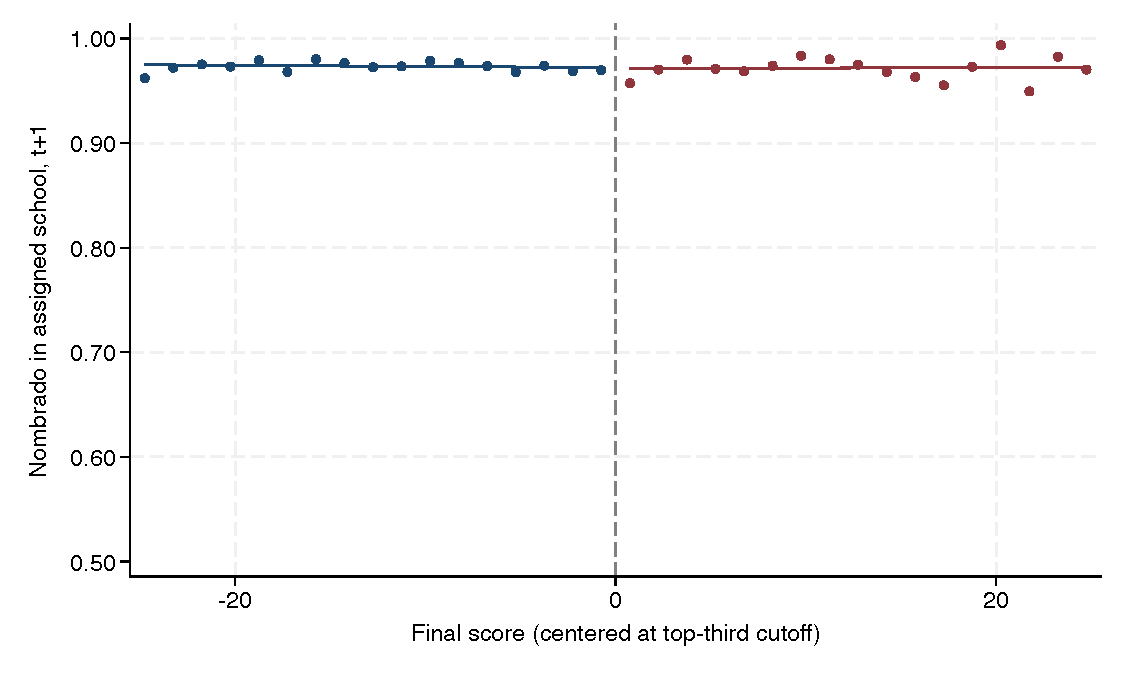
\includegraphics[width=\textwidth]{fig_rf_samesch1.pdf}
\caption{Same school, $t+1$}
\end{subfigure}
\begin{subfigure}[b]{0.42\textwidth}
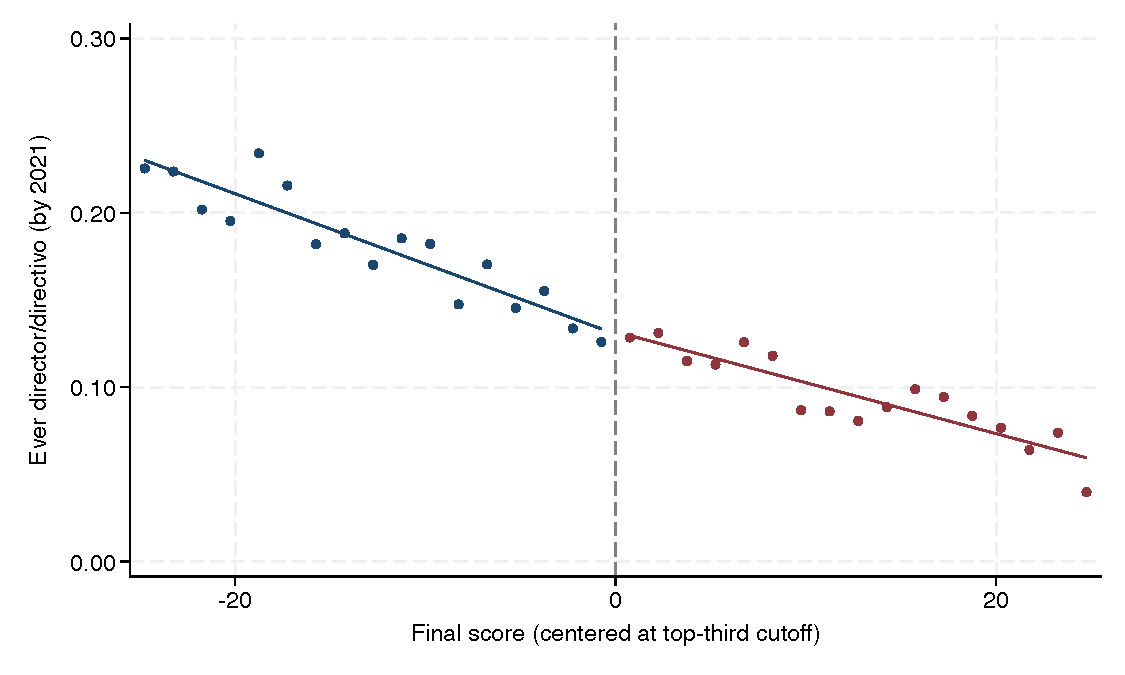
\includegraphics[width=\textwidth]{fig_rf_director.pdf}
\caption{Ever director by 2021}
\end{subfigure}
\caption{Reduced-form discontinuities, pooled concursos. Bins of 1.5 score
points; linear fits weighted by bin size on each side.}
\label{fig:outcomes}
\end{figure}

\begin{figure}[htbp]
\centering
\begin{subfigure}[b]{0.48\textwidth}
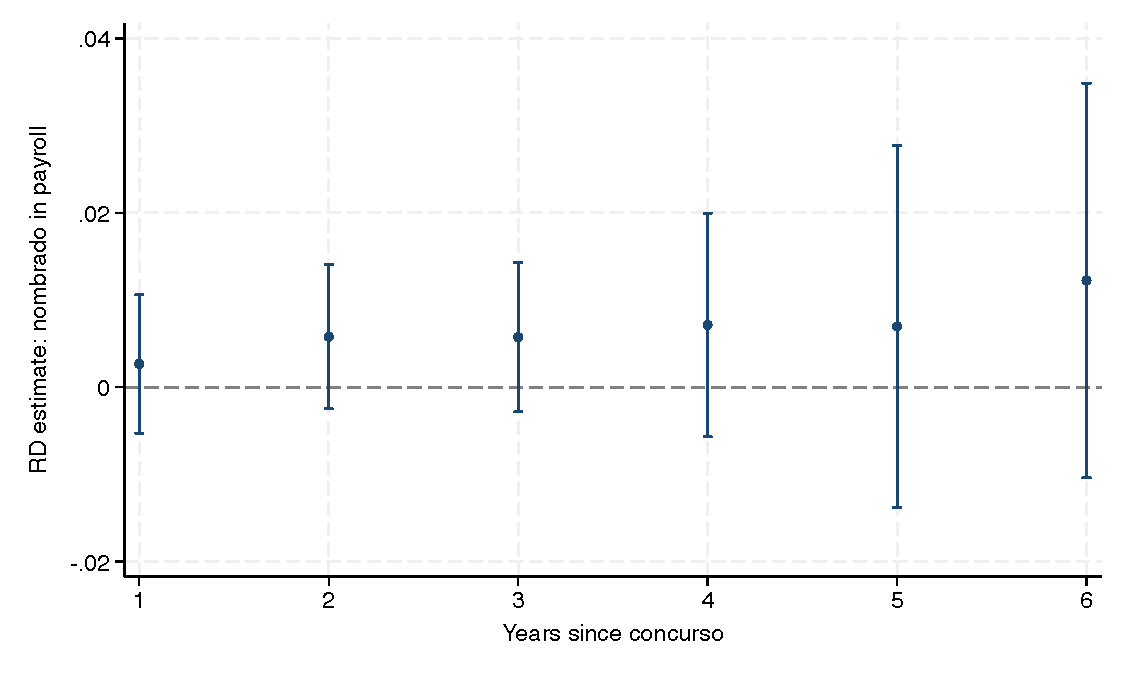
\includegraphics[width=\textwidth]{fig_dynamics_retention.pdf}
\caption{Nombrado in payroll}
\end{subfigure}
\begin{subfigure}[b]{0.48\textwidth}
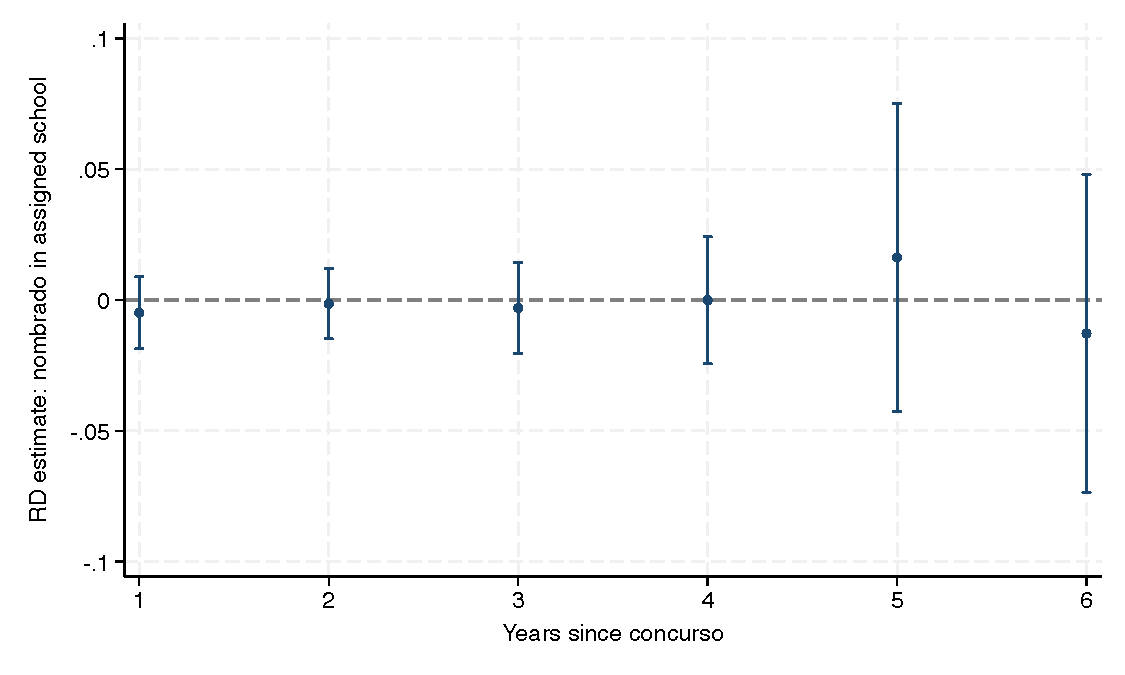
\includegraphics[width=\textwidth]{fig_dynamics_samesch.pdf}
\caption{Nombrado in assigned school}
\end{subfigure}
\caption{RD estimates by years since the concurso (pooled; later horizons
identified by earlier cohorts only). Bars are 95\% confidence intervals.}
\label{fig:dynamics}
\end{figure}

\subsection{Heterogeneity}\label{sec:hetero}

Table~\ref{tab:hetero} splits the donut sample along the rurality and
hardship classification of the assigned plaza---taken from the concurso
plaza database, which records the allowance-relevant categories (urban,
rural 1--3, bilingual, border, VRAEM) for every vacancy in all four
rounds---plus sex, age, baseline employment, and teaching level.
Figure~\ref{fig:hetrural} shows the rural/urban split for same-school
retention, and Figure~\ref{fig:ruralflows} the key comparison within rural
appointees. The last column adds a new outcome built for this section:
teaching (as nombrado) in \emph{any} rural school at $t+2$, using a
school-level rurality lookup constructed from the same plaza database.

The rural/urban contrast is the headline, and with all four cohorts it
sharpens considerably. Among winners assigned to \emph{rural} schools, bonus
recipients are less likely to still be in their assigned school one year
later (\RuralSameschRF~pp, $p=$~\RuralSameschP; \RuralSameschTwoRF~pp at
$t+2$, $p=$~\RuralSameschTwoP), while the urban estimate is a small positive
(+\UrbanSameschRF~pp at $t+1$); the rural--urban difference at $t+1$ is
\RuralUrbanDiff~pp (SE~\RuralUrbanDiffSE, $t=$~\RuralUrbanDiffT). Crucially,
the new rural-system outcome shows that the movers do not relocate to other
rural schools: among rural appointees, the probability of teaching in
\emph{any} rural school at $t+2$ falls by \InruralRuralRF~pp
($p=$~\InruralRuralP, against a control mean of \InruralRuralMean\%), while
their system-level retention is exactly flat (\RuralRetainTwoRF~pp at
$t+2$). The exit is largest where exit is cheapest---Rural~1 schools, the
least remote category (\RuralOneSameschRF~pp at $t+1$,
$p=$~\RuralOneSameschP)---and the degree gradient is not monotone beyond
that. Taken together, the pattern reads as urban drift financed by the
windfall: because the bonus follows the teacher anywhere in the public
system, the S/\,6,000 payments can cover exactly the costs (paperwork,
travel, temporary double residence) of moving out of the hard-to-staff
schools the concurso placed these teachers in.

The mirror image is that the aggregate retention effect is entirely an
urban-appointee phenomenon: system retention at $t+2$ rises by
+\UrbanRetainRF~pp among urban appointees ($p=$~\UrbanRetainP) and not at
all among rural ones. As before, the retention effect is also concentrated
among primary-level teachers (+\PrimRetainRF~pp at $t+2$, $p=$~\PrimRetainP)
and, more weakly, among women (+\FemRetainRF~pp, $p=$~\FemRetainP); there is
no heterogeneity by age or by prior payroll status. The bilingual, VRAEM and
border subsamples are too small for informative estimates at the cutoff
(their confidence intervals span economically large effects of either sign).
Two caveats before we lean on any of this: the subgroup count is now large
enough that a couple of 5--10\% $p$-values are expected under the null, and
the rural/urban split---though predetermined---was chosen after seeing the
aggregate same-school zero. The right discipline is a pre-specified
follow-up: the 2022/2024 cohorts (Section~\ref{sec:dataplan}) provide
out-of-sample replication material once their payroll years accumulate.

\begin{table}[htbp]
\centering
\caption{Heterogeneous RD effects (donut sample, reduced form)}
\label{tab:hetero}
\begin{threeparttable}
\small
\begin{tabular}{lccccc}
\toprule
 & Nombrado & Nombrado & Same school & Same school & Rural school \\
 & $t+1$ & $t+2$ & $t+1$ & $t+2$ & $t+2$ \\
\midrule
All winners & 0.003 & 0.006 & -0.005 & -0.001 & 0.019 \\
 & (0.004) & (0.004) & (0.007) & (0.007) & (0.017) \\
\addlinespace
\emph{Rurality of assigned school} \\
\quad Rural & -0.001 & -0.001 & -0.026** & -0.021* & -0.022* \\
 & (0.007) & (0.006) & (0.013) & (0.013) & (0.012) \\
\quad Urban & 0.005 & 0.012** & 0.005 & 0.014 & 0.001 \\
 & (0.006) & (0.006) & (0.008) & (0.009) & (0.002) \\
\addlinespace
\emph{Degree of rurality} \\
\quad Rural 1 (least remote) & -0.008 & -0.009 & -0.051** & -0.036 & -0.023 \\
 & (0.016) & (0.016) & (0.024) & (0.024) & (0.020) \\
\quad Rural 2 & 0.012 & 0.006 & -0.001 & -0.019 & -0.026 \\
 & (0.011) & (0.011) & (0.020) & (0.026) & (0.025) \\
\quad Rural 3 (most remote) & -0.015 & -0.010 & -0.035 & -0.022 & -0.028 \\
 & (0.011) & (0.010) & (0.020) & (0.024) & (0.023) \\
\addlinespace
\emph{Other hardship categories} \\
\quad Bilingual school & -0.003 & -0.000 & 0.016 & 0.022 & -0.046 \\
 & (0.017) & (0.020) & (0.024) & (0.037) & (0.084) \\
\quad VRAEM school & -0.059 & -0.082 & -0.050 & -0.051 & -0.170 \\
 & (0.048) & (0.073) & (0.033) & (0.047) & (0.118) \\
\quad Border school & 0.008 & 0.009 & 0.018 & 0.015 & 0.150* \\
 & (0.009) & (0.009) & (0.020) & (0.023) & (0.076) \\
\addlinespace
\emph{Sex} \\
\quad Female & 0.004 & 0.008* & -0.005 & 0.001 & 0.023 \\
 & (0.005) & (0.004) & (0.009) & (0.008) & (0.022) \\
\quad Male & -0.002 & 0.002 & -0.004 & -0.006 & 0.016 \\
 & (0.008) & (0.009) & (0.011) & (0.012) & (0.027) \\
\addlinespace
\emph{Age} \\
\quad Below median age & 0.005 & 0.009 & -0.002 & 0.000 & 0.025 \\
 & (0.006) & (0.006) & (0.010) & (0.011) & (0.024) \\
\quad Above median age & 0.001 & 0.003 & -0.006 & -0.003 & 0.016 \\
 & (0.006) & (0.006) & (0.008) & (0.009) & (0.025) \\
\addlinespace
\emph{Baseline employment} \\
\quad In payroll at $t_0$ & 0.004 & 0.006 & -0.007 & -0.003 & 0.014 \\
 & (0.005) & (0.005) & (0.008) & (0.009) & (0.019) \\
\quad New entrant at $t_0$ & -0.001 & 0.008 & 0.004 & 0.013 & 0.064 \\
 & (0.016) & (0.015) & (0.019) & (0.019) & (0.045) \\
\addlinespace
\emph{Teaching level} \\
\quad Inicial & 0.003 & 0.003 & -0.000 & -0.006 & -0.014 \\
 & (0.007) & (0.005) & (0.009) & (0.010) & (0.041) \\
\quad Primaria & 0.012* & 0.016** & -0.009 & 0.005 & 0.010 \\
 & (0.007) & (0.007) & (0.013) & (0.013) & (0.033) \\
\quad Secundaria & -0.002 & 0.002 & -0.002 & -0.003 & 0.039 \\
 & (0.009) & (0.008) & (0.011) & (0.010) & (0.027) \\
\bottomrule
\end{tabular}

\begin{tablenotes}\footnotesize
\item \texttt{rdrobust} local linear estimates by subgroup; standard errors
in parentheses; * $p<0.1$, ** $p<0.05$, *** $p<0.01$ (robust bias-corrected).
Rurality and hardship categories of the assigned plaza come from the concurso
plaza database (all four rounds, 100\% coverage). ``Rural school $t+2$'' is
teaching as nombrado in any rural school two years after the concurso, using
a school-level rurality lookup from the same database. Age split at the
sample median (35). Baseline employment measured in the November payroll of
the concurso year.
\end{tablenotes}
\end{threeparttable}
\end{table}

\begin{figure}[htbp]
\centering
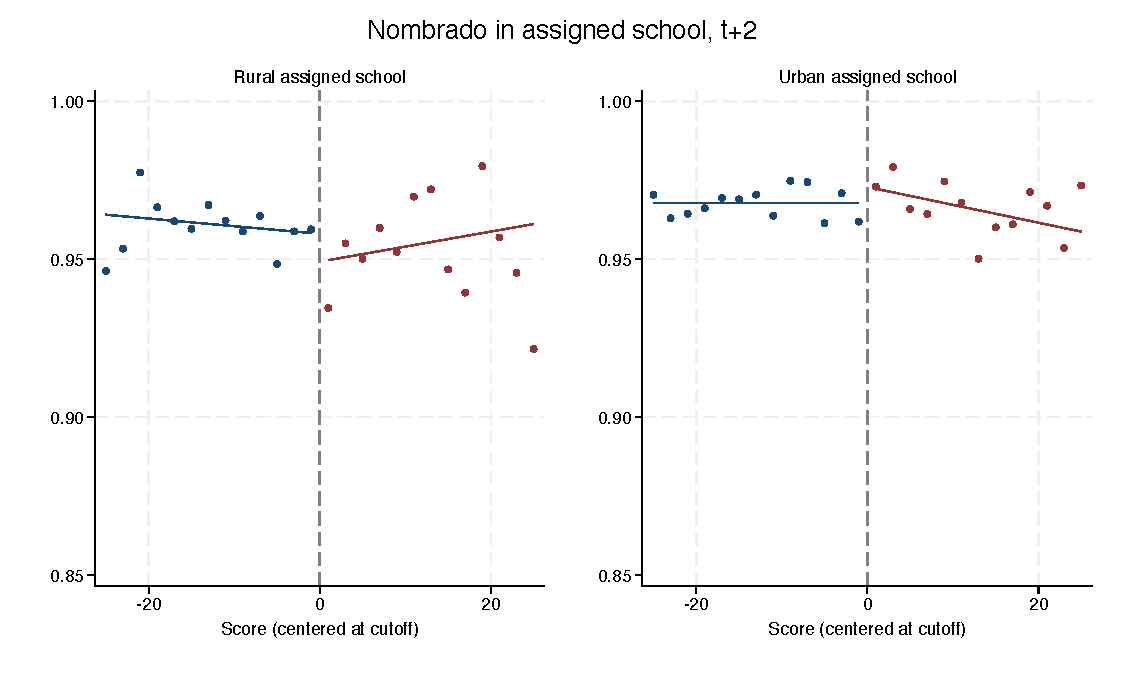
\includegraphics[width=0.9\textwidth]{fig_het_samesch_rural.pdf}
\caption{Same-school retention at $t+2$ by rurality of the assigned school
(2-point bins, donut sample, all four concursos).}
\label{fig:hetrural}
\end{figure}

\begin{figure}[htbp]
\centering
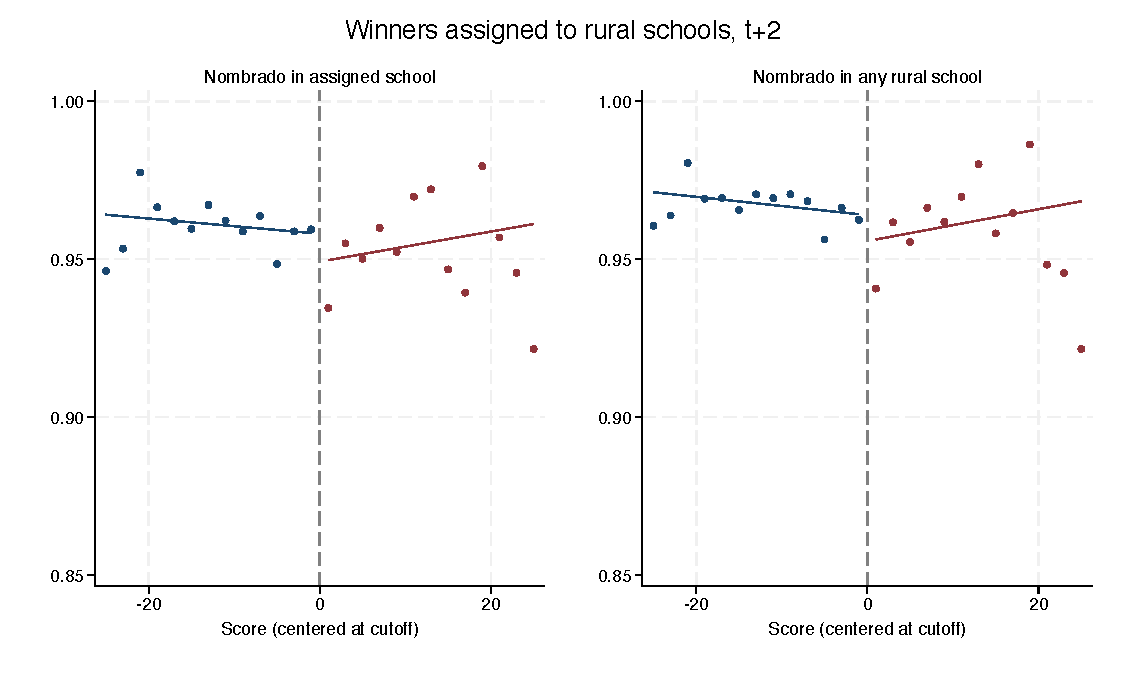
\includegraphics[width=0.9\textwidth]{fig_het_ruralflows.pdf}
\caption{Winners assigned to rural schools: retention in the assigned school
versus in any rural school, $t+2$ (2-point bins, donut sample).}
\label{fig:ruralflows}
\end{figure}

\dataneed{The rurality gap flagged in the previous draft is now closed (the
plaza database covers all cohorts and adds bilingual/border/VRAEM), and the
new any-rural-school outcome already tells us the movers leave the rural
system. What would still sharpen this section: (i) reasignaci\'on (transfer)
records, to see \emph{where} movers go (nearby towns versus across regions)
and \emph{when} within the three payment years; (ii) a continuous hardship
measure (distance to the provincial capital, from school coordinates in the
padr\'on) to replace the four-category classification; (iii) a school-level
rurality \emph{panel} (the padrones de asignaciones, 2014--2026, are in the
Dropbox but not yet synced offline)---our current lookup assigns each school
its latest classification, so reclassifications over time add noise to the
any-rural outcome.}


\subsection{Validity and robustness}

Table~\ref{tab:validity} reports manipulation tests and covariate balance;
Figure~\ref{fig:balance} shows the corresponding balance plots, and
Figure~\ref{fig:density} the raw density. Covariates are smooth through the
cutoff, and the pooled density test does not reject ($p=$~\DensityPooledP).
The 2015 round alone rejects at the 5\% level ($p=0.03$); we read this as an
artifact of the discrete score grid (scores move in half-point steps, and
\texttt{rddensity} is built for continuous running variables) rather than
manipulation---the cutoff is a function of the entire realized score
distribution and was unknowable at the time of scoring---but we will
implement discrete-running-variable diagnostics (e.g., Frandsen's test) in
the next iteration. Table~\ref{tab:robust} shows that the headline estimates
are stable when we include the tie mass point (fuzzy), halve or double the
bandwidth, or use a local quadratic.

\begin{table}[htbp]
\centering
\caption{Validity: density tests and covariate balance}
\label{tab:validity}
\begin{threeparttable}
\begin{tabular}{lcc}
\toprule
 & Statistic / RD estimate & $p$-value \\
\midrule
\multicolumn{3}{l}{\emph{Density tests (rddensity)}} \\
\quad Concurso 2015 & -2.23 & 0.03 \\
\quad Concurso 2017 & 0.13 & 0.89 \\
\quad Concurso 2018 & -0.57 & 0.57 \\
\quad Concurso 2019 & -0.83 & 0.41 \\
\quad Concurso Pooled & -0.78 & 0.43 \\
\midrule
\multicolumn{3}{l}{\emph{Covariate balance (rdrobust, donut)}} \\
\quad Female & 0.003 & 0.83 \\
\quad Age at concurso & 0.179 & 0.50 \\
\quad Assigned school rural & 0.025 & 0.29 \\
\quad Contract teacher, concurso year & -0.015 & 0.35 \\
\quad In payroll, concurso year & -0.015 & 0.25 \\
\bottomrule
\end{tabular}

\begin{tablenotes}\footnotesize
\item Density: \texttt{rddensity} robust bias-corrected test. Balance:
\texttt{rdrobust} estimates on predetermined covariates, donut sample.
\end{tablenotes}
\end{threeparttable}
\end{table}

\begin{table}[htbp]
\centering
\caption{Robustness of the main estimates}
\label{tab:robust}
\begin{threeparttable}
\begin{tabular}{lccc}
\toprule
 & Nombrado $t+1$ & Nombrado $t+2$ & Same school $t+1$ \\
\midrule
Baseline (donut, MSE-optimal bw) & 0.003 & 0.006 & -0.005 \\
 & (0.004) & (0.004) & (0.007) \\
Including ties, fuzzy RD & 0.005 & 0.008 & -0.000 \\
 & (0.005) & (0.005) & (0.006) \\
Half bandwidth & 0.003 & 0.006 & -0.008 \\
 & (0.006) & (0.007) & (0.011) \\
Double bandwidth & 0.002 & 0.004 & -0.001 \\
 & (0.003) & (0.003) & (0.005) \\
Local quadratic & 0.004 & 0.006 & -0.007 \\
 & (0.006) & (0.006) & (0.009) \\
\bottomrule
\end{tabular}

\begin{tablenotes}\footnotesize
\item Each cell is a separate \texttt{rdrobust} estimate; standard errors in
parentheses; * $p<0.1$, ** $p<0.05$, *** $p<0.01$ (robust bias-corrected).
\end{tablenotes}
\end{threeparttable}
\end{table}

\begin{figure}[htbp]
\centering
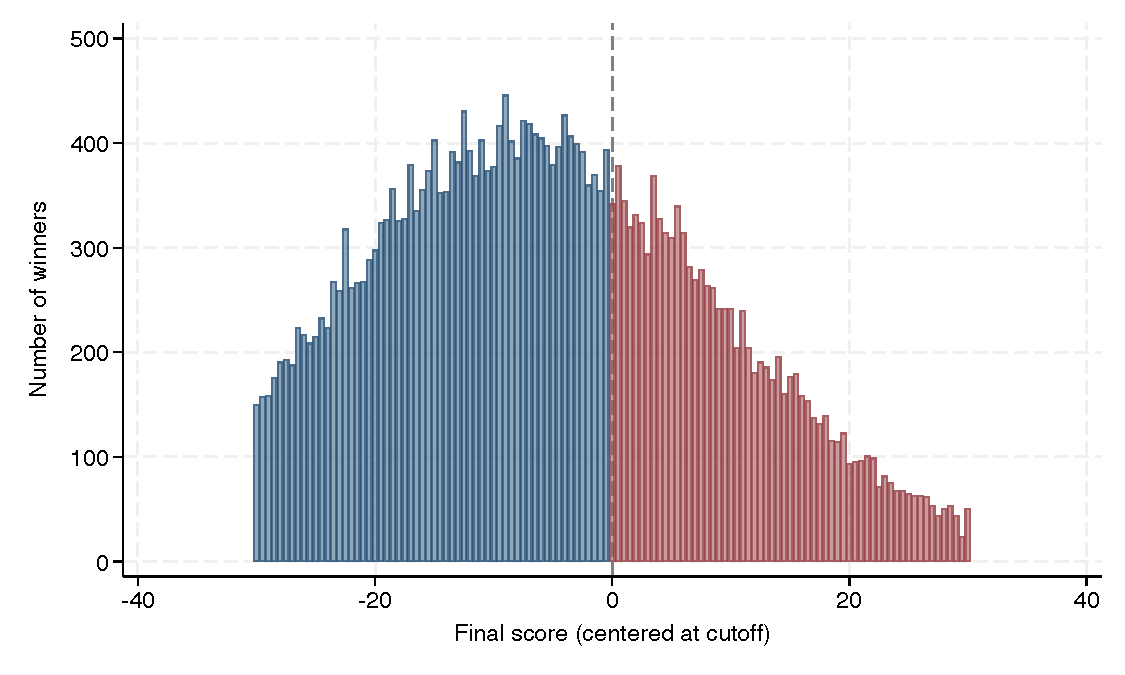
\includegraphics[width=0.6\textwidth]{fig_density_pooled.pdf}
\caption{Density of the running variable (pooled), half-point bins.}
\label{fig:density}
\end{figure}

\begin{figure}[htbp]
\centering
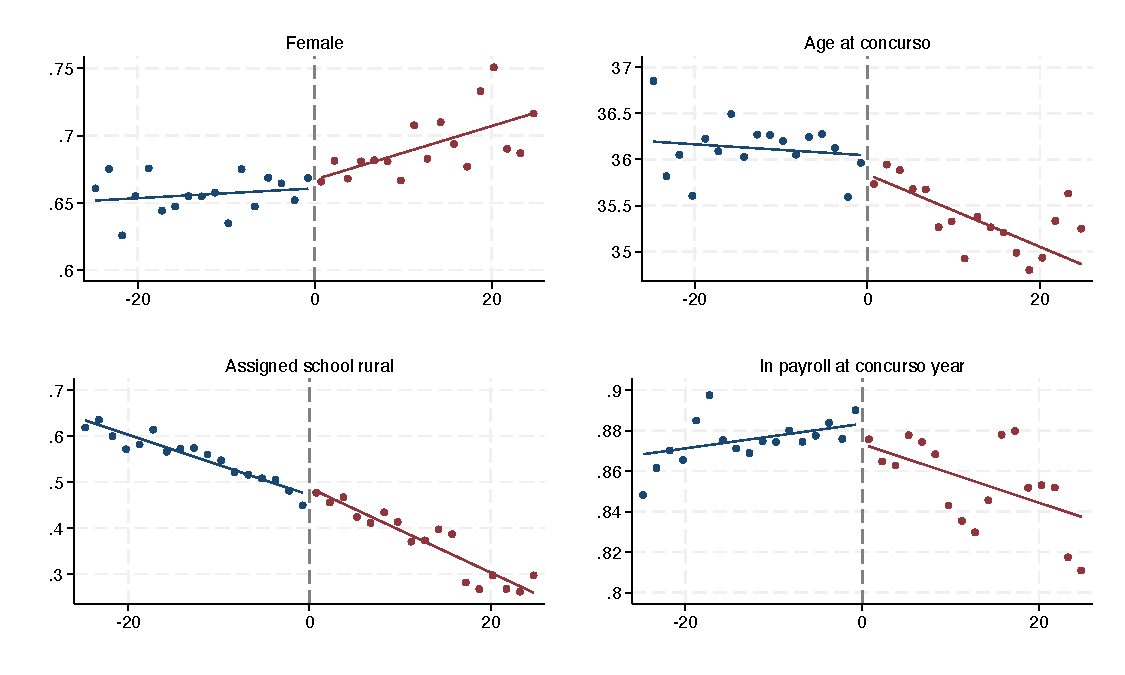
\includegraphics[width=0.85\textwidth]{fig_balance.pdf}
\caption{Covariate balance at the cutoff (pooled, donut sample).}
\label{fig:balance}
\end{figure}

\section{Data acquisition plan: 2022 and 2024 concursos (and beyond)}
\label{sec:dataplan}

Everything missing is public on MINEDU's evaluation portal
(\url{https://evaluaciondocente.perueduca.pe/concursos-y-evaluaciones/evaluaciones-anteriores/}),
organized per concurso with the same architecture as the rounds we already
digitized. We verified the relevant pages for 2022
(\texttt{/nombramiento2022/}) and 2024 (\texttt{/nombramiento24/}): final PUN
results, decentralized-stage results, and winners lists are posted as
per-region PDFs (26 files per set, same layout family as the 2015--2019
sources in \texttt{concursos/source}). The plan, executable by Claude in a
future session:

\begin{enumerate}
\item \textbf{Download} (~1--2 hours, scripted): crawl the results pages for
nombramiento 2022 and 2024 (PUN results, decentralized-stage final results,
ganadores; plus the 2021 round for completeness even though it had no bono)
and store the PDFs under \texttt{concursos/source/} following the existing
convention (\texttt{PUN/2022}, \texttt{N\_descentralizada/2022},
\texttt{N\_ganadores/2022}, etc.), leaving current files untouched.
\item \textbf{Digitize}: extract the tables to CSV with the same
pdf-extraction pipeline used for the bono lists (the PDFs are digital, not
scans; extraction is reliable and verifiable against row counts printed on
the documents).
\item \textbf{Integrate}: append to the cleaned stacked files with
\texttt{concurso==2022/2024} labels, matching the schemas of
\texttt{ganadores\_nombramiento.dta} and \texttt{etapa\_desc\_nombramiento.dta},
with a validation notebook comparing counts to MINEDU's published totals.
\item \textbf{Payroll extension}: the 2015--2021 NEXUS extraction must be
extended to 2022--2025 to measure outcomes for the new cohorts and the
post-bonus years of the 2018--2019 cohorts. Options: (i) the SINAD
information-request route already used for the DIGEDD extraction (the 2025
deliveries in \texttt{nexus/source} suggest requests are being answered);
(ii) MINEDU's open-data portal; (iii) scraping the public NEXUS consultation
tool. We recommend (i), mirroring the exact variable list of the 2015--2021
extraction.
\end{enumerate}

For the 2022/2024 rounds the running variable is the PUN score (per
RVM~118-2021), which is attractive: the PUN is machine-graded, so local
manipulation is even less plausible, and the design extends to a second
incentive regime.

\section{Where this could go: ideas for the paper}\label{sec:ideas}

\begin{enumerate}
\item \textbf{Retention where it binds.} The bonus follows the teacher, not
the school, and the full-sample heterogeneity (Section~\ref{sec:hetero}) now
shows the consequence directly: rural appointees who receive the bonus leave
their assigned school and the rural system while staying in the profession,
and the aggregate retention gain accrues entirely among urban appointees.
The natural paper frames the bono as a test of \emph{unconditional} versus
\emph{location-conditioned} teacher pay: an identical transfer, delivered
without a location string, buys system retention where it is already high
and finances mobility away from where retention binds. Next steps: transfer
(reasignaci\'on) destinations and timing, a continuous hardship gradient,
and out-of-sample replication in the 2022/2024 cohorts.
\item \textbf{Incentive dynamics.} Payments stop after year 3. With payroll
through 2025, we can test for exit spikes when payments end
(2015 cohort: 2019; 2017 cohort: 2021; 2018 cohort: 2022)---an
attractive test separating price effects from selection.
\item \textbf{Career ladders.} The directivo result (+\DirectorRF~pp) can be
validated with the directores concurso files (habilitados/ganadores, which we
have for 2016--2021) and ascenso participation: does a windfall early in the
career finance investment in promotion?
\item \textbf{Student outcomes.} School-level ECE test scores and dropout
(available through 2018/2019) can be linked through the school of service:
does retaining marginal top-third teachers move school outcomes? Power is a
concern given the small retention effect; worth a back-of-the-envelope before
investing.
\item \textbf{The attraction margin.} The RD identifies retention effects,
not attraction. The 2015 introduction (announced before the concurso) and the
2021 rule change (final score $\to$ PUN) are candidate variation for whether
the bonus changed who applies and how they prepare---e.g., a
difference-in-differences on application volumes and applicant quality around
2015, or bunching-style tests on effort in the decentralized stage once the
ranking stopped depending on it in 2021.
\item \textbf{Comparison with location-based bonuses.} Peru also pays
permanent rural/frontier/VRAEM allowances. Contrasting the (unconditional on
location) atracci\'on bonus with location-conditioned pay in the same system
speaks directly to the design of teacher compensation in developing
countries.
\end{enumerate}


\section{Relation to Bobba et al.\ (2026) and Ederer (2026), and two
concrete extensions}\label{sec:related}

Two recent papers study teacher compensation and sorting in exactly our
setting---the Peruvian centralized teacher labor market---using the same
administrative infrastructure (concurso rankings, NEXUS): Bobba, Ederer,
Le\'on-Ciliotta, Neilson and Nieddu (2026; henceforth BELNN), on
\emph{location-based} pay, and Ederer (2026), on the \emph{dynamics} of
teacher--school matching. Neither examines the Bono de Atracci\'on, and the
three-way comparison is unusually clean because the three instruments live in
the same institutional system and are of comparable size.

\textbf{BELNN: person-based versus school-based pay.} BELNN show that wage
rigidity makes teachers sort on non-wage amenities, concentrating competent
teachers in urban schools, and use an RD on the rural wage bonus (a
$\sim$13\% permanent wage increase at remoteness/population cutoffs) to show
that \emph{school-based} pay is powerful on the recruitment margin: new
recruits' competency rises by 0.42$\sigma$ and student math scores by
0.27$\sigma$. Their structural model prices the urban--rural amenity gap: the
most remote schools would need roughly \textbf{S/\,500 per month} to compete
with the average urban school. The Bono de Atracci\'on pays exactly
S/\,500 per month (S/\,6,000 per year) for three years---but attached to the
\emph{person}, not the school. Our RD delivers the missing empirical moment:
the same money, stripped of the location string, buys essentially nothing on
any staffing margin that matters for inequality (no acceptance effect, no
rural retention, negative same-school retention among rural appointees). Two
further points of contact. First, in a static sorting model with additively
separable utility, a person-based transfer that follows the teacher anywhere
does not change \emph{relative} school utilities and should produce exactly
zero sorting effects---our aggregate same-school zero confirms this
prediction out of sample; the \emph{negative} rural effect goes beyond it and
points to a mobility-cost/liquidity channel absent from the baseline model
(cash relaxes the fixed cost of executing a transfer). Second, BELNN find
that even the \emph{school-based} bonus leaves teacher retention unchanged at
their cutoffs (their Table C.7); together with our results, neither
instrument retains teachers in rural schools---location pay works through
recruitment, and person pay works through neither.

\textbf{Ederer: cash and the job ladder.} Ederer's dynamic matching model
rationalizes why urban--rural gaps in teacher effectiveness \emph{widen} with
experience: rural placements are the bottom of a job ladder, and teachers
rematch upward over their careers. His headline counterfactual shows that
\emph{mandating} minimum spells in rural schools backfires through adverse
selection at recruitment, and that negating it would require roughly
S/\,282 per month ($\approx$19\% of base pay). Our heterogeneity results are,
to our knowledge, the first quasi-experimental evidence on the ladder
mechanism itself: an unconditional windfall \emph{accelerates} the climb
(rural appointees leave the assigned school and the rural system while
staying in the profession), and the effect is largest exactly where the
ladder is cheapest to climb (Rural~1 schools). The rural/urban asymmetry in
our estimates is the model's signature: for urban appointees---already near
the top of the ladder---the only margin left is leaving the profession, and
there the bonus \emph{does} retain (+\UrbanRetainRF~pp); for rural appointees
the rematching margin dominates and system retention is flat. The
quantitative coincidence is worth emphasizing: Peru already spends, per
recipient, about \emph{twice} the monthly amount Ederer estimates is needed
to offset the cost of staying in a rural school---it just does not condition
the payment on staying.

\textbf{Extension A (of BELNN): the counterfactual reallocation of the bono
budget.} The bono rounds 2015--2019 disbursed roughly S/\,200 million
(11,147 recipients $\times$ S/\,18,000). BELNN's wage-setting machinery
(their Proposition 1) can price what that budget would buy if converted into
their cost-minimizing, school-based schedule: how much of the rural
effectiveness gap closes when the atracci\'on budget is reallocated from
person-based to location-based pay, holding total cost fixed? Our RD
estimates discipline the model twice---as out-of-sample validation moments
(the zero sorting response to person-based pay; the mobility-cost channel)
and as the empirical description of the status quo policy being replaced.
This is the natural next paper for the BELNN team: same model, same data, a
real S/\,200M policy, and a sharp design.

\textbf{Extension B (of Ederer): pricing a voluntary retention contract.}
Ederer evaluates a \emph{mandate}; the bono suggests its market-based
counterpart: condition the three S/\,6,000 installments on remaining in the
assigned (rural) school, i.e., a voluntary dynamic retention contract rather
than a lock-in. Because participation at each payment date is chosen ex post,
the adverse-selection cost of the mandate is partially avoided, and the
existing budget is approximately the right order of magnitude (S/\,500
$>$ S/\,282 per month). Our RD moments---in particular the negative
same-school and any-rural effects and their timing relative to the payment
window---identify the income effect on mobility that his model needs to
simulate this contract credibly. The policy question the extension answers:
how much rural retention (and downstream student achievement) does the
\emph{same} S/\,200M buy under (i) the current unconditional design, (ii) a
stay-in-school-conditioned design, and (iii) BELNN's recruitment-margin
schedule?

For the standalone RD paper, this positioning also settles the framing: the
Bono de Atracci\'on is the empirical test of the \emph{person-based} corner
of the teacher compensation design space, completing a triptych whose other
corners---school-based pay (BELNN) and mobility restrictions (Ederer)---are
already written.

\appendix

\section{Bono beneficiary lists: file-by-file inventory}\label{app:lists}

\begin{itemize}
\item \texttt{bono\_atraccion\_2015.csv} (2,702 rows). Columns: names, DNI,
\emph{puntaje final}, region, \emph{orden de m\'erito}. Header of the source
PDF states the top-third rule over final scores among winners with a
nombramiento resolution and adjudicated plaza. Fully consistent with the
2015 ganadores file (100\% DNI match).
\item \texttt{bono\_atraccion\_2017.csv} (3,617 rows). Columns include
\emph{puntaje concurso} and \emph{puntaje bono}; they differ for 58 rows, and
where they differ the concurso score equals the bono score times a
bonification factor (1.10/1.15/1.25). Best guess (verified against
decentralized-stage bonification sub-scores): the bono ranking uses the
unbonified score. Six DNIs on the list do not appear in our ganadores file;
unresolved, plausibly late plaza adjudications.
\item \texttt{bono\_atraccion\_2018.csv} (3,351 rows) and
\texttt{bono\_atraccion\_2019.csv} (1,489 rows). Single \emph{puntaje total}
column; three DNIs each unmatched to ganadores. At the 2018 cutoff score only
4 of 99 winners received the bonus---the strongest evidence that ties at the
cutoff were broken by an unobserved criterion (the norm suggests the order of
the underlying ranking components; we drop the mass point).
\item \texttt{bono\_atraccion\_2022.csv} (9,999 rows) and
\texttt{bono\_atraccion\_2024.csv} (8,210 rows). Single \emph{puntaje} column
on a $\sim$150--190 scale, consistent with the PUN-only ranking of
RVM~118-2021; includes a \texttt{dni\_flag} for rows where the DNI failed a
checksum in digitization (to re-verify against source PDFs). Not yet usable
for RD without the 2022/2024 concurso rankings (Section~\ref{sec:dataplan}).
\item \textbf{Open questions for MINEDU/colleagues:} (i) the exact
tie-breaking rule at the cutoff score; (ii) whether the 87 above-cutoff
non-recipients are indeed protocol exclusions (no validated nombramiento at
the cut date; prior beneficiaries); (iii) for 2022/2024, the exact validation
date defining the eligible pool.
\end{itemize}

\section{Code and file map}

All code lives in \texttt{Claude/Principals/Bono de atraccion/}:
\texttt{code/01\_build\_rd\_dataset.do} (RD base),
\texttt{code/02\_build\_outcomes.do} (NEXUS outcomes),
\texttt{code/03\_analysis.do} (estimates and figures),
\texttt{code/04\_make\_tables.py} (tables and the numbers in this document),
with logs in \texttt{logs/} and derived data in \texttt{data/}
(\texttt{rd\_analysis.dta} is the analysis file). Source folders under
\texttt{Teachers Peru/Data} are treated as read-only.

\end{document}
